\chapter{Μηχανική μάθηση και συστήματα συστάσεων}
\label{chap2}
\sloppy
\section{Μηχανική μάθηση}
\renewcommand\figurename{Εικόνα}
\begin{figure}[!htb]
	%\vspace{2px}%
	\centering
	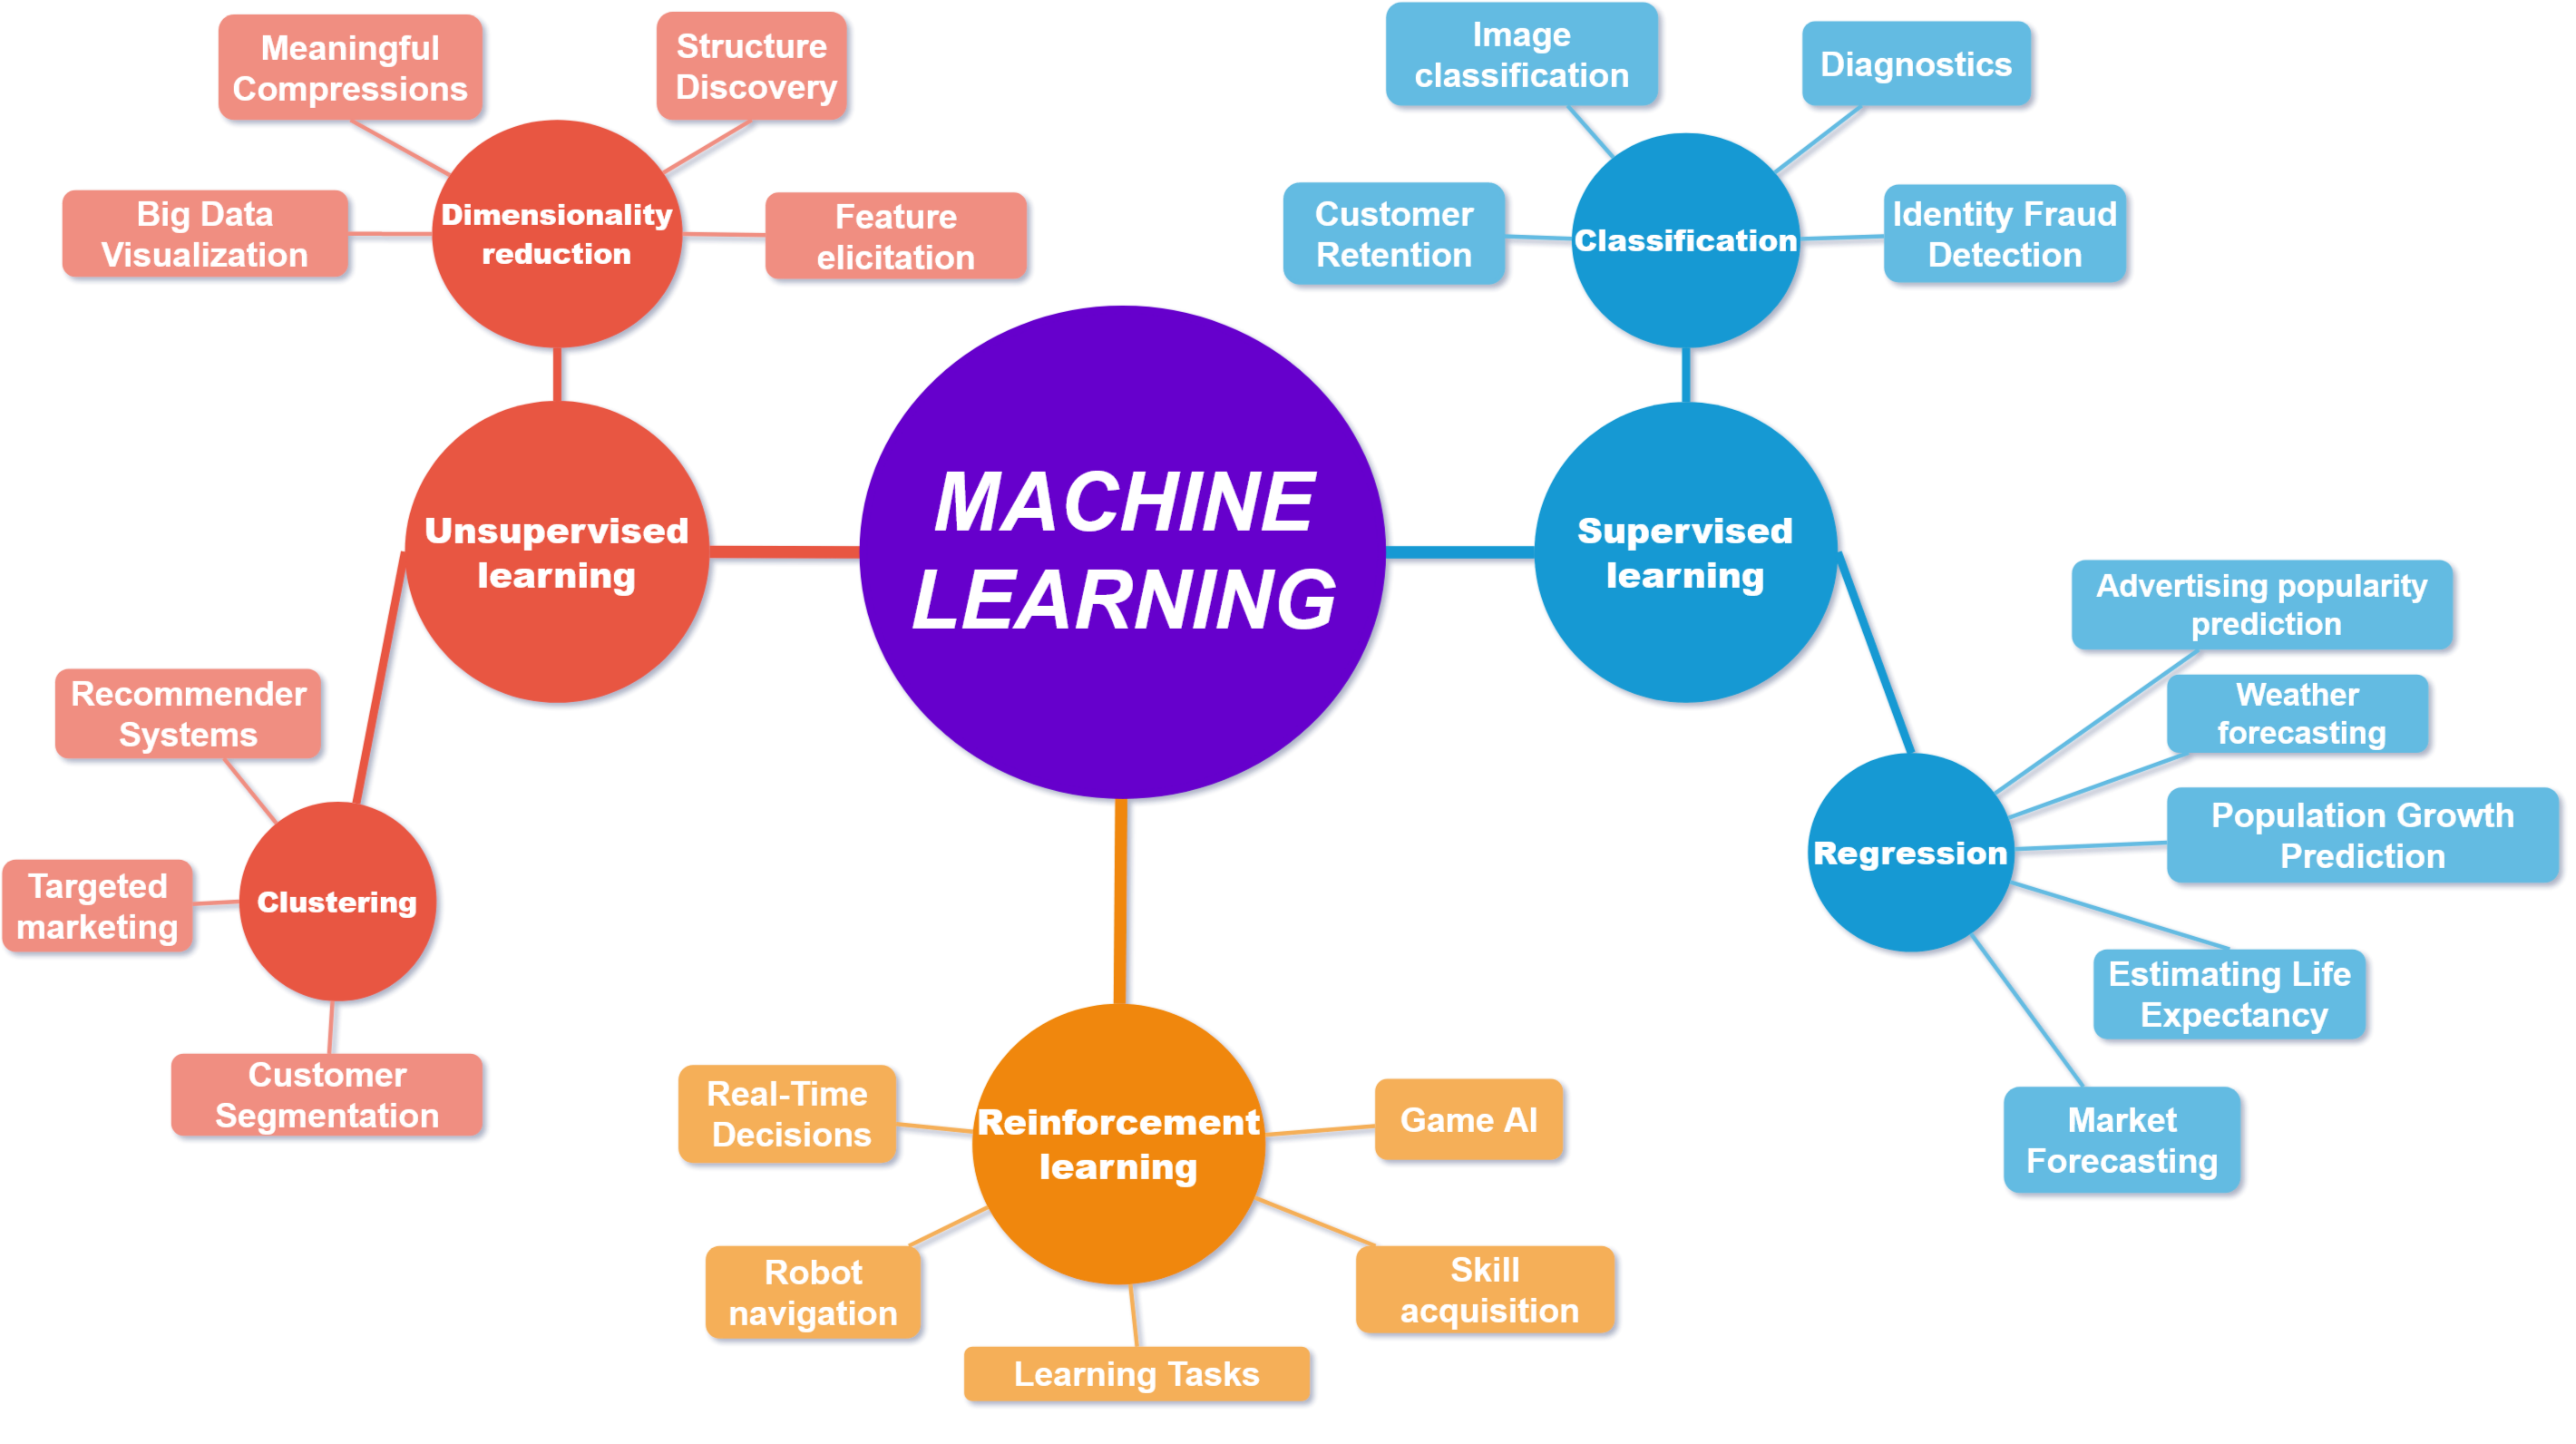
\includegraphics[width=\linewidth]{drawio3.png}
	\caption{Είδη μηχανικής μάθησης}
	\label{fig:ml}
\end{figure}
\noindent Η μηχανική μάθηση είναι ένα από τα πιο ραγδαίως αναπτυσσόμενα πεδία τα τελευταία χρόνια με εφαρμογές στη βιοπληροφορική, στην οικονομία (τραπεζικός τομέας, ανάλυση μετοχών), στις τηλεπικοινωνίες, στις ιατρικές διαγνώσεις, στην τεχνολογία λογισμικού, στο μάρκετινγκ, στην αναγνώριση ομιλίας, στη ρομποτική και σε αρκετά ακόμη πεδία. Αποτελεί ένα υποπεδίο της τεχνητής νοημοσύνης, ενώ έχουν αναπτυχθεί αρκετοί ορισμοί για αυτό. Ένας από τους πρώτους και πιο απλούς ορισμούς δόθηκε από τον Samuel\cite{samuelStudiesMachineLearning1959a} «Η μηχανική μάθηση αποτελεί πεδίο μελέτης που δίνει στους υπολογιστές την ικανότητα να μαθαίνουν, χωρίς να έχουν ρητά προγραμματιστεί», ενώ ένας πιο επίσημος ορισμός δίνεται από τον Mitchell \cite{mitchellMachineLearning1997}: «Ένα πρόγραμμα υπολογιστή λέμε ότι μαθαίνει από την εμπειρία Ε ως προς κάποια κλάση εργασιών Τ και μέτρο απόδοσης Ρ, αν η απόδοσή του σε εργασίες από το Τ, όπως μετριέται από το Ρ, βελτιώνεται μέσω της εμπειρίας Ε.».
Όπως περιγράφεται στο \cite{maloneARTIFICIALINTELLIGENCEFUTURE} η συνάρτηση ενός συστήματος μηχανικής μάθησης μπορεί να είναι \textbf{περιγραφική (descriptive)}, το οποίο σημαίνει ότι το σύστημα χρησιμοποιεί τα δεδομένα για να περιγράψει τι έχει συμβεί, \textbf{προγνωστική (predictive)}, που σημαίνει ότι το σύστημα χρησιμοποιεί τα δεδομένα για να προβλέψει τι θα συμβεί ή \textbf{προστακτική (prescriptive)}, όπου το σύστημα χρησιμοποιεί τα δεδομένα για να δημιουργήσει προτάσεις σχετικές με το ποια ενέργεια θα πρέπει να γίνει.
Οι αλγόριθμοι μηχανικής μάθησης εντάσσονται σε τρεις κύριες κατηγορίες, ανάλογα με το είδος της μάθησης όπως φαίνεται και στην Εικόνα \ref{fig:ml}. Οι κατηγορίες αυτές είναι η επιβλεπόμενη μηχανική μάθηση \en {(supervised learning)}, η μη-επιβλεπόμενη \en {(unsupervised learning)} και η ενισχυμένη 
\en {(reinforcement learning)} και περιγράφονται αναλυτικά στην επόμενη υποενότητα. Η περιγραφή αυτών των εννοιών έγινε ύστερα από εμβριθή μελέτη των πιο κλασικών βιβλίων για αυτό το είδος \cite{burkovHundredPageMachineLearning2019}, \cite{hastie2009elements}



\subsection{Κατηγορίες αλγορίθμων μάθησης}
\begin{figure}[H]
	%\vspace{2px}%
	\centering
	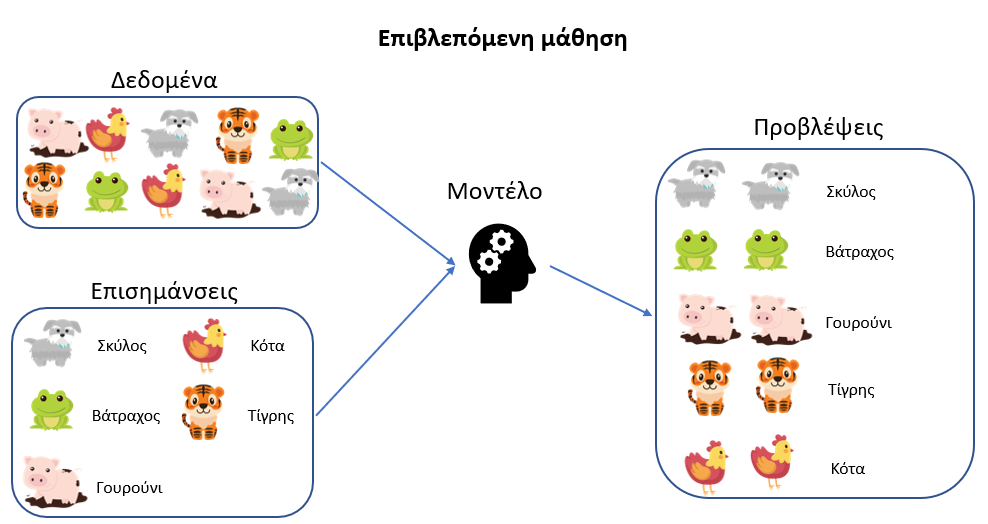
\includegraphics[width=\linewidth]{sl1.png}
	\caption{Επιβλεπόμενη μάθηση}
	\label{fig:su}
\end{figure}
\noindent\textbf{Επιβλεπόμενη μάθηση}
\\
Στην επιβλεπόμενη μηχανική μάθηση (supervised learning) οι αλγόριθμοι δέχονται ως είσοδο δεδομένα τα οποία έχουν επισημανθεί με ετικέτες (labelled data) και τα χρησιμοποιούν για την εκπαίδευσή τους. Ονομάζεται επιβλεπόμενη διότι στην εκπαίδευση λαμβάνει μέρος και κάποιος ειδικός, ο οποίος διακρίνει πότε ο αλγόριθμος παράγει σωστά αποτελέσματα και προβαίνει στις κατάλληλες διορθώσεις του αλγορίθμου έως ότου παραχθούν σωστά αποτελέσματα.
Η επιβλεπόμενη μάθηση διαιρείται περαιτέρω σε δύο κύριες κατηγορίες: την παλινδρόμηση (regression) και την κατηγοριοποίηση (classification).
\newpage
\begin{itemize}
\item[$\blacksquare$]
\noindent\textbf{Κατηγοριοποίηση}\\
Σύμφωνα με την περιγραφή που δίνει η Dunham στο \cite{dunhamDataMiningIntroductory2002}, ένα πρόβλημα κατηγοριοποίησης χρησιμοποιεί μια συνάρτηση αντιστοίχισης (mapping function) για την αντιστοίχιση μεταβλητών εισόδου (X) σε διακριτές μεταβλητές εξόδου (Y). Σε ένα πρόβλημα κατηγοριοποίησης ο αλγόριθμος λαμβάνει επισημασμένα δεδομένα ως είσοδο για την εκπαίδευσή του και παράγει ένα μοντέλο το οποίο αν πάρει ως είσοδο μη-προσημασμένα δεδομένα δίνει ως πρόβλεψη επισημάνσεις για αυτά. Μια επισήμανση ανήκει σε ένα πεπερασμένο σύνολο κλάσεων. Εάν το πλήθος των κλάσεων είναι ίσο με δύο, για παράδειγμα έστω δύο κλάσεις για να περιγράψουμε την κατάσταση της υγείας ενός ανθρώπου («άρρωστος», «υγιής»), τότε έχουμε δυαδική κατηγοριοποίηση (binary classification), εάν υπάρχουν περισσότερες από δύο κλάσεις τότε έχουμε κατηγοριοποίηση πολλών κλάσεων (multiclass classification). Οι πιο γνωστοί αλγόριθμοι κατηγοριοποίησης είναι οι Support Vector Machines (SVM), Naïve Bayes, Decision Tree, Random Forest, Κ-Nearest Neighbors (KNN) και οι αλγόριθμοι νευρωνικών δικτύων.
\item[$\blacksquare$] \noindent\textbf{Παλινδρόμηση}\\
Η παλινδρόμηση είναι μια στατιστική διαδικασία πρόβλεψης, η οποία εν αντιθέσει με την κατηγοριοποίηση παράγει ως πρόβλεψη συνεχείς μεταβλητές \cite{hastie2009elements}. Χρησιμοποιείται κυρίως για την κατανόηση της σχέσης που υπάρχει ανάμεσα σε ανεξάρτητες και εξαρτημένες μεταβλητές, δηλαδή σε προβλήματα όπως η πρόβλεψη της θερμοκρασίας, προβλέψεις σχετικές με την οικονομία και η πρόβλεψη χρονοσειρών. Οι πιο δημοφιλείς αλγόριθμοι παλινδρόμησης είναι οι Logistic Regression, Linear Regression, Ridge Regression και Polynomial Regression.
\\
\end{itemize}
\begin{figure}[H]
	%\vspace{2px}%
	\centering
	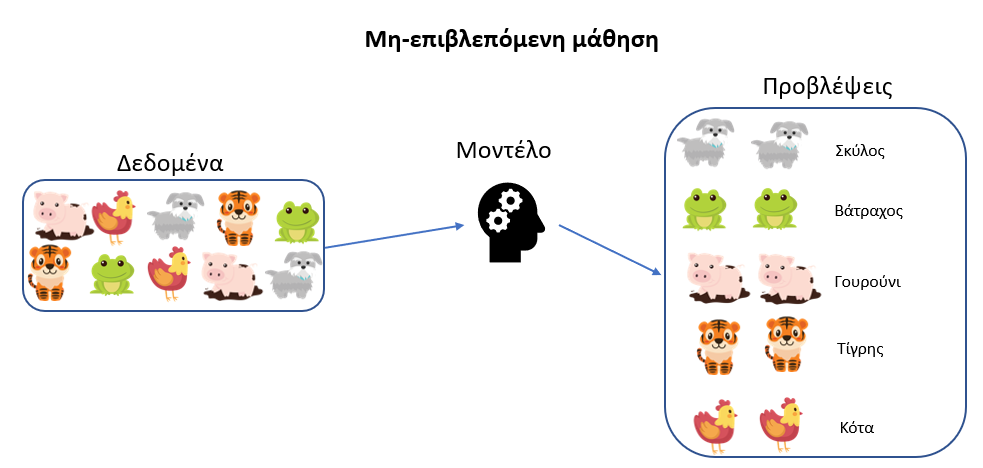
\includegraphics[width=\linewidth]{unsl.png}
	\caption{Μη-επιβλεπόμενη μάθηση}
	\label{fig:unsl}
\end{figure}


\noindent\textbf{Μη-επιβλεπόμενη μάθηση}\\
Η μη επιβλεπόμενη μηχανική μάθηση (unsupervised learning) δέχεται ως είσοδο δεδομένα χωρίς επισήμανση (unlabeled data) και κατηγοριοποίηση και χρησιμοποιεί αλγόριθμους για την εξαγωγή σημαντικών χαρακτηριστικών που απαιτούνται για την επισήμανση, την ταξινόμηση και την κατηγοριοποίηση των δεδομένων σε πραγματικό χρόνο, χωρίς ανθρώπινη παρέμβαση. Ο κύριος στόχος της μη-επιβλεπόμενης μάθησης είναι η ανακάλυψη προτύπων. Όταν ένα μοντέλο μάθει να αναπτύσσει πρότυπα, μπορεί εύκολα να προβλέψει πρότυπα για κάθε νέο σύνολο δεδομένων με τη μορφή συστάδων. Ακολούθως περιγράφονται ορισμένες εργασίες (tasks) μη-επιβλεπόμενης μάθησης.
\begin{itemize}
	\item[$\blacksquare$] \noindent\textbf{Συσταδοποίηση (Clustering)}\\
Είναι ο διαχωρισμός των σημείων ενός συνόλου δεδομένων σε κατηγορίες που ονομάζονται συστάδες (clusters).  Κάθε συστάδα περιέχει δεδομένα που έχουν παρόμοια χαρακτηριστικά. Η διαφορά της συσταδοποίησης από την κατηγοριοποίηση είναι ότι δεν υπάρχουν προκαθορισμένες κατηγορίες. Υπάρχουν αρκετοί αλγόριθμοι συσταδοποίησης: K-Means, BIRCH, DBSCAN, Gaussian Mixture Models (GMM) είναι ορισμένοι από αυτούς. Τέλος, αξίζει να αναφερθεί πως η συσταδοποίηση είναι μια πάρα πολύ χρήσιμη τεχνική για εργασίες όπως η ανάλυση δεδομένων, τα συστήματα συστάσεων, η μείωση της διαστατικότητας (dimensionality reduction), οι μηχανές αναζήτησης, η κατάτμηση εικόνας (image segmentation) και αρκετές ακόμη.
\item[$\blacksquare$] \textbf{Μείωση διαστατικότητας (dimensionality reduction)}\\
Όπως μαρτυράει και το όνομα, στόχος εδώ είναι η μείωση των διαστάσεων των δεδομένων. Η πιο συνηθισμένη προσέγγιση που ακολουθείται εδώ είναι η Principal Component Analysis (PCA)

\end{itemize}


\noindent\textbf{Ημι-επιβλεπόμενη μάθηση}\\
Η ημι-επιβλεπόμενη μάθηση (semi-supervised learning) είναι ένας συνδυασμός της επιβλεπόμενης και της μη-επιβλεπόμενης μάθησης. Πιο αναλυτικά, ορισμένοι αλγόριθμοι μπορούν να διαχειριστούν μεγάλη ποσότητα μη-επισημασμένων δεδομένων και αρκετά μικρή ποσότητα επισημασμένων δεδομένων. \\


\noindent\textbf{Ενισχυμένη μάθηση}\\
Η ενισχυμένη μηχανική μάθηση (Reinforcement machine learning) \cite{kaelblingReinforcementLearningSurvey1996} έχει αρκετές ομοιότητες με την επιβλεπόμενη μηχανική μάθηση. Η κύρια διαφορά τους ωστόσο, είναι ότι η ενισχυμένη μάθηση δεν χρησιμοποιεί επισημασμένα δεδομένα για την εκπαίδευση του μοντέλου, αλλά ο agent (ο μαθητής - \en{learner} και υπεύθυνος λήψης αποφάσεων) παρατηρεί το περιβάλλον (environment), επιλέγει και εκτελεί μια ενέργεια (action) και μαθαίνει μέσω ενός συστήματος επιβράβευσης/ποινών. Το περιβάλλον αφού λάβει την επιλεγμένη ενέργεια και την κατάσταση (state) του agent ως είσοδο, παράγει ως έξοδο, για κάθε σωστή ενέργεια μια ανταμοιβή (positive reward) και για κάθε λανθασμένη μια ποινή (negative reward), καθώς και την επόμενη κατάσταση. Ο agent επιλέγει την επόμενη ενέργειά του, μέσω μια στρατηγικής (policy), η οποία στην πραγματικότητα είναι μια συνάρτηση, με βάση την τρέχουσα κατάσταση στην οποία βρίσκεται, που παίρνει ως είσοδο. Ο στόχος ενός agent είναι να επιλέξει τη βέλτιστη στρατηγική ώστε να μεγιστοποιήσει τις ανταμοιβές που λαμβάνει. Σε αυτή την κατεύθυνση ο agent αξιοποιεί (exploit) την γνώση που ήδη έχει ώστε να λάβει μια ανταμοιβή και εξερευνά (explore) το περιβάλλον ώστε να λάβει επιπλέον πληροφορίες για αυτό και να μεγιστοποιήσει αυτή την ανταμοιβή. Οι εφαρμογές της ενισχυμένης μηχανικής μάθησης είναι πολλές και ποικίλες:  επεξεργασία φυσικής γλώσσας (Natural Language Processing - NLP), ρομποτική, βαθιά μάθηση,  υγειονομική περίθαλψη, χρηματοοικονομικά, ηλεκτρονικά παιχνίδια, είναι μόνο μερικές από αυτές.

\subsection{Εκπαίδευση και αξιολόγηση της απόδοσης των μοντέλων μηχανικής μάθησης}
\noindent Αφού καθοριστεί η κατηγορία στην οποία ανήκει το πρόβλημα μηχανικής μάθησης που καλούμαστε να αντιμετωπίσουμε και επιλεγεί ο καταλληλότερος αλγόριθμος, ακολουθεί η εκπαίδευση του αλγορίθμου στα δεδομένα που θα του παρέχουμε ως είσοδο. Πριν από αυτό όμως, κρίνεται αναγκαία μια προεπεξεργασία των δεδομένων. Μια από τις πιο γνωστές και συχνότερα χρησιμοποιούμενες στρατηγικές, είναι η διάσπαση του συνόλου δεδομένων που έχουμε στη διάθεσή μας σε δύο υποσύνολα. Το μεγαλύτερο θα είναι το σύνολο εκπαίδευσης (training set) το οποίο δίνεται ως είσοδος στον αλγόριθμο μηχανικής μάθησης και στο οποίο θα γίνει η εκπαίδευση του αλγορίθμου μας και το άλλο θα είναι το σύνολο δοκιμής (test set) στο οποίο θα γίνει η δοκιμή της απόδοσης του μοντέλου ύστερα από την εκπαίδευσή του. Τα πιο συνηθισμένα ποσοστά διάσπασης είναι 80\% ή 70\% του αρχικού συνόλου δεδομένων να αποτελεί το σύνολο εκπαίδευσης και το 30\% ή 20\% να αποτελεί το σύνολο δοκιμής. Σε ορισμένες περιπτώσεις η διαδικασία της δοκιμής της απόδοσης του μοντέλου γίνεται σε δύο βήματα και για αυτόν τον λόγο χρειάζεται και ένα ακόμη σύνολο, τo σύνολο επικύρωσης (validation set). Στο πρώτο βήμα το σύνολο αυτό χρησιμοποιείται για την αξιολόγηση και την επιλογή του βέλτιστου μοντέλου και τη ρύθμιση υπερπαραμέτρων (hyperparameter tuning), ενώ στο δεύτερο βήμα χρησιμοποιείται το σύνολο δοκιμής όπως ακριβώς και πριν. 

\noindent Σε αυτήν την υποενότητα παρουσιάζονται ορισμένες μετρικές αξιολόγησης της απόδοσης των μοντέλων μηχανικής μάθησης, κάτι που κρίνεται απαραίτητο προκειμένου να γίνουν πιο κατανοητές ορισμένες έννοιες που θα παρουσιαστούν στις επόμενες ενότητες.

\noindent Το πρώτο πράγμα που μας ενδιαφέρει συνήθως όσον αφορά την αξιολόγηση της απόδοσης ενός μοντέλου μηχανικής μάθησης είναι η \textit{ακρίβεια (accuracy)}:
\begin{align*}
 \text{Ακρίβεια} = \frac{\text{αριθμός σωστών προβλέψεων}}{\text{συνολικός αριθμός προβλέψεων}}
\end{align*}
Όταν έχουμε να επιλύσουμε προβλήματα κατηγοριοποίησης, τότε υπάρχουν τέσσερα πιθανά αποτελέσματα που μπορεί να προκύψουν, πρώτα όμως ας δούμε ένα πολύ συγκεκριμένο παράδειγμα από την καθημερινή ζωή. Έστω ένα διαγνωστικό τεστ το οποίο μας δείχνει αν κάποιος νοσεί από κορονοϊό ή όχι. Ορίζεται ως κλάση των θετικών (positive class) το γεγονός κάποιος άνθρωπος να νοσεί από κορονοϊό και ως κλάση των αρνητικών (negative class) το γεγονός κάποιος άνθρωπος να μην νοσεί από κορονοϊό. Πιο γενικά, στην κλάση των θετικών έχουμε δεδομένα που έχουν κάποιο χαρακτηριστικό, ενώ αντίθετα στην κλάση των αρνητικών έχουμε δεδομένα που δεν έχουν κάποιο χαρακτηριστικό. Σε αυτό το σημείο μπορούμε να εξετάσουμε τα τέσσερα αποτελέσματα που μπορεί να προκύψουν από τις προβλέψεις ενός μοντέλου κατηγοριοποίησης:

\bigskip

\noindent \textbf{Αληθώς θετικά – True positives (TP):} το μοντέλο προβλέπει επιτυχώς τη θετική (positive) κλάση. Ο ασθενής νοσεί από κορονοϊό και το τεστ βγαίνει θετικό.

\bigskip

\noindent \textbf{Ψευδώς θετικά – \en{False positives (FP)}:} το μοντέλο προβλέπει εσφαλμένα τη θετική (positive) κλάση. Ο ασθενής δεν νοσεί από κορονοϊό και το τεστ βγαίνει θετικό.

\bigskip

\noindent \textbf{Αληθώς αρνητικά – \en{True negatives (TN)}:} το μοντέλο προβλέπει επιτυχώς την αρνητική (negative) κλάση. Ο ασθενής δεν νοσεί από κορονοϊό και το τεστ βγαίνει αρνητικό.

\bigskip

\noindent \textbf{Ψευδώς αρνητικά – False negatives (FN):} το μοντέλο προβλέπει εσφαλμένα την αρνητική (negative) κλάση. Ο ασθενής νοσεί από κορονοϊό και το τεστ βγαίνει αρνητικό.

\bigskip

\noindent \textbf{Ποσοστό αληθώς θετικών - True Positive Rate (TPR):} ονομάζεται και Recall ή sensitivity και είναι το ποσοστό των σωστών προβλέψεων στην κλάση των θετικών, δηλαδή όταν ένας άνθρωπος νοσεί πραγματικά, πόσο συχνά προβλέπει ότι νοσεί; 

$$ 
TPR = \frac{\text{{\textit{αριθμός  των αληθώς θετικών}}}}{\text{{αριθμός των αληθώς θετικών + αριθμός των ψευδώς αρνητικών  }}} =1-FNR
$$

\bigskip

\noindent\textbf{Ποσοστό ψευδώς θετικών - False Positive Rate (FPR):} το ποσοστό των λανθασμένων προβλέψεων στην κλάση των θετικών, δηλαδή όταν ένας άνθρωπος δεν νοσεί πραγματικά, πόσο συχνά προβλέπει ότι νοσεί; 

\medskip

$$ FPR = \frac {\text{αριθμός των ψευδώς θετικών}}{\text{αριθμός των ψευδώς θετικών + αριθμός των αληθώς αρνητικών}} =1-TNR
$$
\\
\noindent
\textbf{Ποσοστό αληθώς αρνητικών - True Negative Rate (TNR):} είναι γνωστό και ως specificity και περιγράφει το ποσοστό των σωστών προβλέψεων στην κλάση των αρνητικών, δηλαδή όταν ένας άνθρωπος δεν νοσεί πραγματικά, πόσο συχνά προβλέπει ότι δεν νοσεί; 
\\
$$ TNR= \frac{\text{ αριθμός των αληθώς αρνητικών}}{\text{αριθμός των αληθώς αρνητικών + αριθμός των ψευδώς θετικών}}=1-FPR $$
\\
\noindent
\textbf{Ποσοστό ψευδώς αρνητικών - False Negative Rate (FNR):} το ποσοστό των λανθασμένων προβλέψεων στην κλάση των αρνητικών, δηλαδή όταν ένας άνθρωπος νοσεί πραγματικά, πόσο συχνά προβλέπει ότι δεν νοσεί; Είναι γνωστό και ως ποσοστό αποτυχιών (miss rate). 
$$ FNR= \frac{\text{ αριθμός των ψευδώς αρνητικών}}{\text{αριθμός των αληθώς θετικών + αριθμός των ψευδώς αρνητικών}}=1-TPR $$
\newpage
\section{Συστήματα συστάσεων}
\label{rec_sys_chap}
\begin{figure}[H]
	%\vspace{2px}%
	\centering
	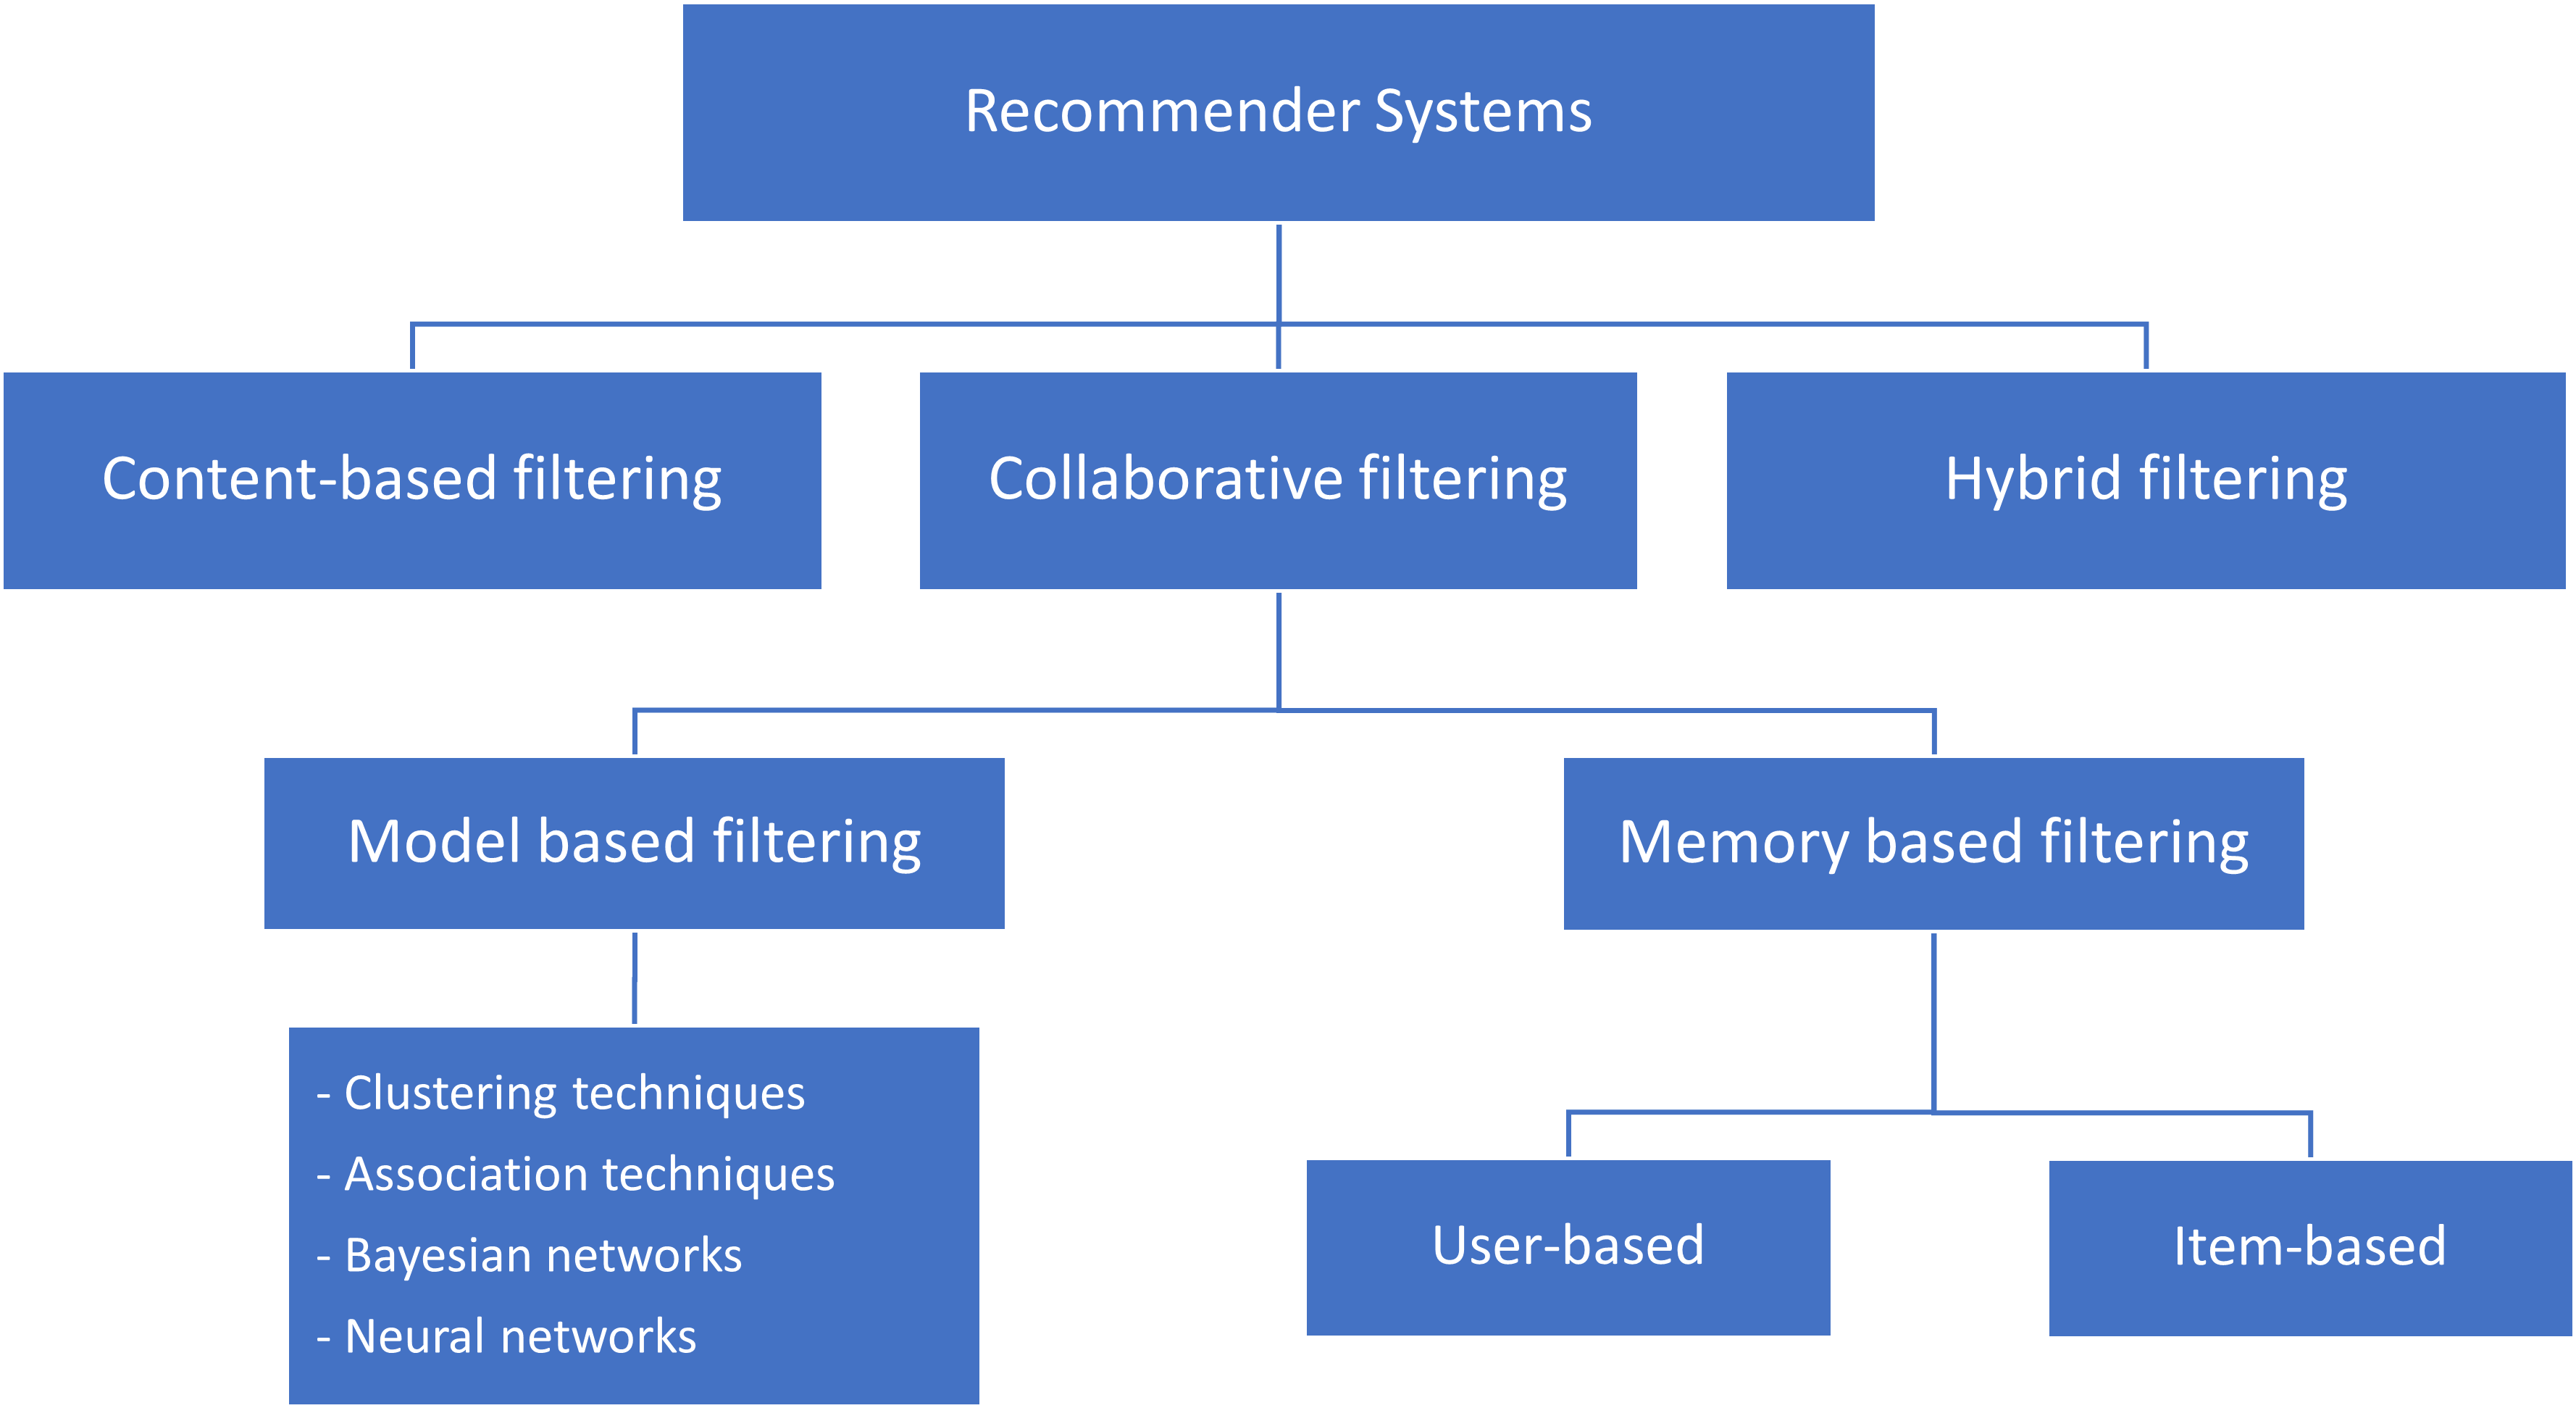
\includegraphics[width=\linewidth]{recsys_handmade.png}
	%	\caption[Κατηγορίες αλγορίθμων συστημάτων συστάσεων]{Κατηγορίες αλγορίθμων συστημάτων συστάσεων [Πηγή: \url{https://silo.ai/ai-recommender-systems}] }
	\caption{Κατηγορίες αλγορίθμων συστημάτων συστάσεων}
	\label{fig:rstypes}
\end{figure}
\noindent
Στην υποενότητα αυτή θα γίνει μια αναφορά στην έννοια των συστημάτων συστάσεων, στα είδη αυτών καθώς και στα πιο συνηθισμένα προβλήματα που εντοπίζονται σε αυτά. Η ανάλυση που ακολουθεί βασίζεται στα βιβλία \cite{falkPracticalRecommenderSystems2019}, \cite{aggarwalRecommenderSystems2016}, \cite{ricciRecommenderSystemsHandbook2011} στα οποία μπορείτε να ανατρέξετε, αν επιθυμείτε να εμβαθύνετε περισσότερο.\\\\
Ως σύστημα συστάσεων (recommendation ή recommender system ή RecSys εν συντομία) ορίζεται το σύστημα όπου οι άνθρωποι παρέχουν προτάσεις ως εισόδους οι οποίες έπειτα συγκεντρώνονται και κατευθύνονται σε συγκεκριμένους παραλήπτες \cite{resnickRecommenderSystems1997}. Αυτός ήταν ένας από τους πρώτους ορισμούς που δόθηκαν για τα συστήματα συστάσεων. Οι βασικές οντότητες που υπάρχουν σε αυτά τα συστήματα είναι οι χρήστες (users) και τα αντικείμενα (items). Η χρήση των συστημάτων συστάσεων έχει αυξηθεί κατακόρυφα τελευταία στο χώρο του διαδικτύου, καθώς τα συστήματα αυτά χρησιμοποιούνται στον χώρο του ηλεκτρονικού εμπορίου, στα κοινωνικά δίκτυα, σε συστήματα παροχής υπηρεσιών ψυχαγωγίας, στις μηχανές αναζήτησης και σε πολλές ακόμη υπηρεσίες.
Ιδιαίτερη σημασία σε ένα σύστημα συστάσεων έχει η συλλογή των δεδομένων από τους χρήστες, δηλαδή η λήψη feedback από αυτούς. Υπάρχουν δύο κύριοι τρόποι για να γίνει αυτό:
 \begin{enumerate}
		\item \textbf{Implicit feedback (έμμεση ανάδραση) \cite{oardImplicitFeedbackRecommender1998}:} σε αυτή την περίπτωση δεν υπάρχει άμεση εμπλοκή του χρήστη στην αξιολόγηση των αντικειμένων. Το σύστημα συλλέγει στοιχεία σχετικά με τον χρήστη όπως είναι το ιστορικό αναζήτησης, τα κλικ που έχει κάνει, τα αντικείμενα που έχει δει ή/και έχει αγοράσει και το προφίλ του (ηλικία, φύλο κτλ.). Μέσω αυτών των στοιχείων το σύστημα έχει τη δυνατότητα να προβλέψει ποια είναι τα αντικείμενα που ενδιαφέρουν τον χρήστη, ώστε να δημιουργήσει τις κατάλληλες συστάσεις για αυτόν. Στην έμμεση ανάδραση οι τιμές στο μητρώο χρηστών-αντικειμένων αντιστοιχούν στην σιγουριά (confidence) που έχουμε για μια παρατήρηση που έχει γίνει για την σχέση ενός χρήστη με ένα αντικείμενο.
		\item \textbf{Explicit feedback (ρητή ανάδραση):} οι χρήστες, εν αντιθέσει με το implicit feedback, παρέχουν αξιολογήσεις σε αντικείμενα που έχουν δει ή έχουν αγοράσει, είτε δίνοντας κάποια βαθμολογία, συνήθως σε κλίμακα 1 έως 5 ή 5 έως 10, είτε δηλώνοντας απλά αν τους άρεσε ή όχι κάποιο αντικείμενο (like και dislike), δηλαδή παρέχοντας μια δυαδική αξιολόγηση (binary rating), είτε -πιο σπάνια- επιλέγοντας μια γραπτή αξιολόγηση (ordinal rating) όπως στα ερωτηματολόγια («καθόλου», «λίγο», «πολύ», «πάρα πολύ»). Στη ρητή ανάδραση οι τιμές στο μητρώο χρηστών-αντικειμένων αντιστοιχούν σε προτιμήσεις (preferences) των χρηστών για τα αντικείμενα.
\end{enumerate}
Φυσικά σε πολλές περιπτώσεις υπάρχει και ο συνδυασμός του implicit και του explicit feedback, δημιουργώντας ένα υβριδικό feedback.\\
\noindent Υπάρχουν τρεις κύριοι τύποι συστημάτων συστάσεων και άρα τρεις τύποι αλγορίθμων, όπως φαίνεται και στην Εικόνα \ref{fig:rstypes}, οι οποίοι περιγράφονται αναλυτικά στην επόμενη υποενότητα.\\

\noindent \subsection[Συστήματα βασισμένα στη συνεργατική διήθηση\\ (Collaborative-filtering systems)]{Συστήματα βασισμένα στη συνεργατική διήθηση (Collaborative-filtering systems)}\label{collab}

\noindent Τα συστήματα αυτά, βασίζονται στην υπόθεση ότι αν σε κάποιον χρήστη αρέσει ένα αντικείμενο Α, και σε έναν άλλο χρήστη αρέσει το αντικείμενο Α μαζί με κάποιο άλλο αντικείμενο Β, τότε ο πρώτος χρήστης είναι αρκετά πιθανό να ενδιαφέρεται και για το αντικείμενο Β. Οπότε, βασίζεται σε παλιές αλληλεπιδράσεις μεταξύ χρηστών και αντικειμένων, ώστε να προβλέψει νέες. Είναι μια αρκετά δημοφιλής προσέγγιση, η οποία χρησιμοποιείται από τα μεγαλύτερα και τα πιο ευρέως χρησιμοποιούμενα συστήματα, όπως η Αmazon, το YouTube, το Netflix, το LinkedIn και το Spotify. Υπάρχουν δύο τύποι μεθόδων που χρησιμοποιούνται στα συστήματα που βασίζονται στη συνεργατική μάθηση:
\begin{itemize}
	\item[$\blacksquare$] 	\textbf{Μέθοδοι με βάση το περιεχόμενο (memory-based methods):} γνωστές και ως μέθοδοι με βάση τη γειτονιά (neighborhood-based) ή ευρετικές (heuristic-based) μέθοδοι. Βασίζονται στην υπόθεση ότι παρόμοιοι χρήστες εμφανίζουν παρόμοια μοτίβα συμπεριφοράς ως προς την αξιολόγηση των αντικειμένων και ότι παρόμοια αντικείμενα λαμβάνουν παρόμοιες αξιολογήσεις. Στις μεθόδους με βάση το περιεχόμενο, οι αξιολογήσεις που έχουν υποβάλλει οι χρήστες σε ορισμένα αντικείμενα και έχουν αποθηκευτεί στο σύστημα, χρησιμοποιούνται απευθείας για την πρόβλεψη αξιολογήσεων για νέα αντικείμενα. Υπάρχουν δύο τρόποι για να γίνει αυτό.
	\begin{itemize}
		\item
		Ο πρώτος είναι η\textbf{ διήθηση χρήστη προς χρήστη (user-user ή user based filtering)}\cite{resnickGroupLensOpenArchitecture1994}, η οποία για ένα συγκεκριμένο χρήστη U, βρίσκει K χρήστες οι οποίοι έχουν παρόμοια ενδιαφέροντα με αυτόν, με βάση την ομοιότητα των αξιολογήσεων, και προτείνει αντικείμενα στον χρήστη U τα οποία άρεσαν σε αυτούς τους χρήστες. Οι K παρόμοιοι αυτοί χρήστες είναι οι γείτονες του χρήστη U. Η εύρεση της ομοιότητας δύο αντικειμένων γίνεται υπολογίζοντας κάποια μετρική ομοιότητας, όπως για παράδειγμα η μετρική συνημιτόνου (cosine similarity), η μετρική Chebyshev και πολλές άλλες. Μέσω αυτών των μετρικών βρίσκονται οι K πλησιέστεροι γείτονες κάθε αντικειμένου. Η μαθηματική περιγραφή των όσων περιγράψαμε δίνεται από τον τύπο:
		\begin{align}
			\widehat{r_{u_{1}i}}= μ_{u_1} + \frac{\sum_{j\in N_u^k\left(i\right)}\mathrm{sim}\left(u_1,u_2\right)\cdot r_{u_2j}}{\sum_{j\in P_u^k\left(i\right)}\mathrm{sim}\left(u_1,u_2\right)}
		\end{align}
	 όπου $ sim\left(u_1,u_2\right)  $ είναι η συνάρτηση που υπολογίζει την ομοιότητα ανάμεσα στο χρήστη $ u_1 $ για τον οποίο θέλουμε να δημιουργήσουμε τις συστάσεις και σε έναν χρήστη $ u_2 $, $ μ_u $ είναι η μέση αξιολόγηση του χρήστη u: $ μ_u = \frac{\sum_{k \in I_{u}}r_{uk}}{|I_{u}|} $ με $ I_{u} $ το σύνολο των δεικτών των αντικειμένων που έχει αξιολογήσει ο χρήστης u, $ P_{u_1}^k\left(i\right) $ είναι το σύνολο των k πλησιέστερων χρηστών στον χρήστη $ u_1 $  και $r_{u_2j} $ η αξιολόγηση που έχει δώσει ο χρήστης  $ u_2 $ στο αντικείμενο j.
		\item
		Αντίθετα, στον δεύτερο τρόπο, τη \textbf{διήθηση αντικείμενο προς αντικείμενο (item-item ή item-based filtering)}\cite{lindenAmazonComRecommendations2003}, για τη δημιουργία συστάσεων για έναν χρήστη U δημιουργείται ένα σύνολο παρόμοιων αντικειμένων με όσα έχει αλληλεπιδράσει θετικά ο χρήστης U. Ως θετική αλληλεπίδραση ορίζουμε μια θετική αξιολόγηση, μια αγορά ενός αντικειμένου ή ακόμη και ένα κλικ, δηλαδή μια προβολή του αντικειμένου από τον χρήστη. Σε αυτό το σημείο θα πρέπει να επισημάνουμε πως δύο αντικείμενα θεωρούνται παρόμοια αν οι περισσότεροι χρήστες έχουν αλληλεπιδράσει με παρόμοιο τρόπο και με τα δύο αυτά αντικείμενα, για παράδειγμα έστω ένα σύνολο δεδομένων από μια επιχείρηση ηλεκτρονικού εμπορίου, αν οι περισσότεροι χρήστες που αγόρασαν το προϊόν “Sony PlayStation 5”, αγόρασαν επίσης και το βιντεοπαιχνίδι “Fifa 21”, τότε προκύπτει το συμπέρασμα ότι αυτά τα δύο προϊόντα είναι παρόμοια. Η αξιολόγηση γίνεται υπολογίζοντας αποστάσεις (distances) ανάμεσα σε αυτά τα αντικείμενα. Η μέθοδος αυτή για ένα αντικείμενο Ι βρίσκει χρήστες στους οποίους άρεσε αυτό το αντικείμενο, καθώς και άλλα αντικείμενα τα οποία άρεσαν στους συγκεκριμένους ή σε «παρόμοιους» χρήστες. Το όνομα αυτής της μεθόδου προκύπτει από το γεγονός ότι παίρνει ως είσοδο αντικείμενα και δίνει ως έξοδο άλλα αντικείμενα ως προτάσεις.  
		Η πρόβλεψη υπολογίζεται με παρόμοιο τρόπο με την μέθοδο διήθησης χρήστη προς χρήστη:
		\begin{align}
		\widehat{r_{ui}}= μ_u + \frac{\sum_{j\in N_u^k\left(i\right)}\mathrm{sim}\left(i,j\right)\cdot r_{uj}}{\sum_{j\in N_u^k\left(i\right)}\mathrm{sim}\left(i,j\right)}
		\end{align}
	    όπου $ sim(i, j)  $ είναι η συνάρτηση που υπολογίζει την ομοιότητα ανάμεσα στο αντικείμενο i και στο αντικείμενο j, $ μ_u $ είναι η μέση αξιολόγηση του χρήστη u: $ μ_u = \frac{\sum_{k \in I_{u}}r_{uk}}{|I_{u}|} $ με $ I_{u} $ το σύνολο των δεικτών των αντικειμένων που έχει αξιολογήσει ο χρήστης u, $ N_u^k\left(i\right) $ είναι το σύνολο των αντικειμένων στην γειτονιά που ο χρήστης u έχει αξιολογήσει και $ r_{uj} $ η αξιολόγηση που έχει δώσει ο χρήστης u στο αντικείμενο j.
	 \end{itemize}
 \item[$\blacksquare$] 	\textbf{Μέθοδοι με βάση το μοντέλο (model-based):} σε αυτήν την περίπτωση τα μοντέλα συνεργατικής διήθησης παρέχουν συστάσεις στους χρήσεις μέσω αλγορίθμων μηχανικής μάθησης. O στόχος είναι να εκπαιδεύσουμε τα μοντέλα, προκειμένου να μας δώσουν ως προβλέψεις λίστες συστάσεων. Συναντάμε τρεις κύριους τύπους: α) Matrix Factorization (MF) β) υλοποιήσεις που βασίζονται σε τεχνικές βαθιάς μάθησης (κυρίως σε νευρωνικά δίκτυα) και γ)  αλγόριθμους συσταδοποίησης (clustering based).
\end{itemize}
Στην παρούσα εργασία θα μας απασχολήσουν κυρίως τα συστήματα που βασίζονται στη συνεργατική διήθηση και πιο συγκεκριμένα τα συστήματα βασισμένα στο μοντέλο, επομένως όπως γίνεται αντιληπτό θα δοθεί λίγη περισσότερη έμφαση στην ανάλυση αυτών.
Στη συνέχεια αυτής της υποενόητας θα αναφέρουμε τις κυριότερες κατηγορίες αλγορίθμων.
\newpage
\noindent
\textbf{Μοντέλα λανθανόντων παραγόντων (Latent factor models) }
\\
Στη γραμμική άλγεβρα ένα μητρώο (matrix) $ m\times n $ ορίζεται ως ένας ορθογώνιος πίνακας αριθμών, συμβόλων ή εκφράσεων, διατεταγμένων σε m γραμμές και n στήλες \cite{beauregardFirstCourseLinear1973}. Ένα διάνυσμα (vector) είναι μια ειδική περίπτωση ενός μητρώου, που έχει μία μόνο στήλη. Στα συστήματα συστάσεων κάθε αντικείμενο αναπαρίσταται από ένα διάνυσμα, με τόσες γραμμές όσοι και οι χρήστες, όπου κάθε κελί (i, j) περιέχει την αξιολόγηση του χρήστη i για το αντικείμενο j. Ένα μητρώο αξιολογήσεων (rating matrix) $  R\in{\mathbb{R}\ }^{m\times\ n} $ αποτελείται από όλα τα διαθέσιμα αντικείμενα, πλήθους n, και όλους τους διαθέσιμους χρήστες, πλήθους m, ενός συνόλου δεδομένων, με άλλα λόγια στο μητρώο αποθηκεύονται όλα τα διανύσματα που προαναφέρθηκαν.\\
Το μητρώο αξιολογήσεων μπορεί να περιέχει χιλιάδες ή ακόμη και εκατομμύρια γραμμές και στήλες. Η μεγάλη αύξηση των διαστάσεων έχεις ως συνέπεια την εκθετική αύξηση του χώρου διαστάσεων και αυξάνει κατά πολύ την αραιότητα (sparsity) των δεδομένων, προκαλώντας μια πληθώρα προβλημάτων. Αυτό το φαινόμενο έχει γίνει γνωστό από τον Richard E. Bellman \cite{bellman1957dynamic} ως «κατάρα της διαστατικότητας» (curse of dimensionality). Στα μοντέλα λανθανόντων παραγόντων, χρησιμοποιούνται τεχνικές μείωσης της διαστατικότητας (dimensionality reduction) για τον υπολογισμό του μητρώου δεδομένων (data matrix). Πιο συγκεκριμένα, η βασική υπόθεση σε αυτά είναι η αξιοποίηση των συσχετίσεων που υπάρχουν ανάμεσα σε αρκετές γραμμές και στήλες του μητρώου δεδομένων, δηλαδή ανάμεσα σε χρήστες και αντικείμενα. Μέσω αυτής της υπόθεσης, είναι εφικτή η προσέγγιση του μητρώου δεδομένων με αρκετά καλή ακρίβεια από ένα μητρώο μικρότερης τάξης. Το ερώτημα εδώ είναι πως επιτυγχάνεται αυτό.
\\\\
Έστω ένα δείγμα από D-διάστατα πραγματικά διανύσματα, που έχουν παραχθεί από μια άγνωστη κατανομή. Η κατανομή στο χώρο δεδομένων γίνεται στην πραγματικότητα εξαιτίας της παρουσίας ενός μικρού αριθμού μεταβλητών (L<D) που δρουν σε συνδυασμό μεταξύ τους, για παράδειγμα ταινίες που έχουν θετική συσχέτιση μεταξύ τους, οι μεταβλητές αυτές ονομάζονται λανθάνουσες (latent variables) ή κρυφές (hidden) καθώς δεν είναι άμεσα ορατές αλλά η εύρεσή τους γίνεται από έναν αλγόριθμο. Με αυτόν τον τρόπο δημιουργείται ένα σημείο στον λανθάνοντα χώρο σύμφωνα με μια προηγούμενη κατανομή και αντιστοιχίζεται στο χώρο δεδομένων με μια ομαλή αντιστοίχιση. Αυτό έχει ως αποτέλεσμα τη δημιουργία ενός L-διάστατου υπόχωρου στον χώρο δεδομένων. Προκειμένου να επεκταθεί αυτό σε ολόκληρο τον D-διάστατο χώρο δεδομένων, ορίζουμε ένα μοντέλο θορύβου (σφάλματος). Το μοντέλο λανθανουσών μεταβλητών ορίζεται από την αντιστοίχιση από τον λανθάνοντα χώρο στον χώρο δεδομένων και το μοντέλο θορύβου σε χώρο δεδομένων. Οι παράμετροι ενός τέτοιου μοντέλου συνήθως βελτιστοποιούνται με τη χρήση ενός κριτηρίου μέγιστης πιθανοφάνειας (maximum likelihood) με χρήση του αλγόριθμου Μεγιστοποίησης Προσδοκίας (Expectation Maximization - EM). Η μείωση των διαστάσεων επιτυγχάνεται με τον ορισμό μιας αντίστροφης αντιστοίχισης από τον χώρο δεδομένων στον λανθάνοντα χώρο, έτσι ώστε σε κάθε σημείο δεδομένων να εκχωρείται ένας αντιπρόσωπος στον λανθάνοντα χώρο.  Υπάρχουν αρκετές τεχνικές μείωσης της διαστατικότητας, η πιο ευρέως χρησιμοποιούμενη από αυτές είναι η παραγοντοποίηση μητρώου.

\noindent
\begin{itemize}
	\item \textbf{Παραγοντοποίηση μητρώου (Matrix Factorization)}


\noindent Όπως προαναφέρθηκε, ένα ζήτημα που προκύπτει με το μητρώο αξιολογήσεων R είναι ότι στις περισσότερες περιπτώσεις δεν υπάρχει αλληλεπίδραση μεταξύ όλων των χρηστών και όλων των αντικειμένων και ως εκ τούτου ορισμένα κελιά του μητρώου αξιολογήσεων μένουν κενά, δημιουργώντας ένα αραιό μητρώο. Το ερώτημα που τίθεται επομένως είναι πώς γεμίζουμε αυτά τα κενά κελιά.\\
Μια λύση σε αυτό αποτελεί η μείωση της διαστατικότητας μέσω της παραγοντοποίησης μητρώου \cite{korenMatrixFactorizationTechniques2009}. Η παραγοντοποίηση είναι η μέθοδος με την οποία διασπάμε μια μεγάλη ποσότητα, για παράδειγμα έναν μεγάλο αριθμό, σε μικρότερες ποσότητες οι οποίες ονομάζονται παράγοντες (factors). Εάν αυτή η ποσότητα δεν είναι ένας αριθμός, αλλά ένα μητρώο, στην περίπτωσή μας το μητρώο R, τότε αυτό διασπάται σε δύο μητρώα μικρότερων διαστάσεων από το R, το $ U\in{\mathbb{R}\ }^{m\times k} $ και το $  V\in{\mathbb{R}\ }^{n\times k} $. Το μητρώο R παραγοντοποιείται ως εξής:\\

\qquad\	\qquad\ \qquad\ \qquad\ \qquad\ \qquad\ \qquad\ \quad\ $ R\approx UV^\top $
\\\\
Το ένα από τα δύο μητρώα είναι το μητρώο χρήστη (user matrix) και το άλλο το μητρώο αντικειμένου (item matrix). Οι γραμμές των δύο μητρώων ονομάζονται λανθάνοντες παράγοντες (latent factors) και οι στήλες λανθάνοντα διανύσματα (latent vectors). Κάθε γραμμή του μητρώου χρήστη είναι ένα διάνυσμα το οποίο περιέχει k λανθάνοντες παράγοντες οι οποίοι περιγράφουν τον χρήστη u και αντίστοιχα κάθε γραμμή του μητρώου αντικειμένου είναι ένα διάνυσμα το οποίο περιέχει k λανθάνοντες παράγοντες οι οποίοι περιγράφουν το αντικείμενο i. 
Κάθε αξιολόγηση $ r_{ui} $ του χρήστη u στο αντικείμενο i στο R υπολογίζεται μέσω του εσωτερικού γινομένου των δύο διανυσμάτων: $ r_{ui}=\ p_uq_i $. 
\begin{figure}[!htb]
%\vspace{2px}%
\centering
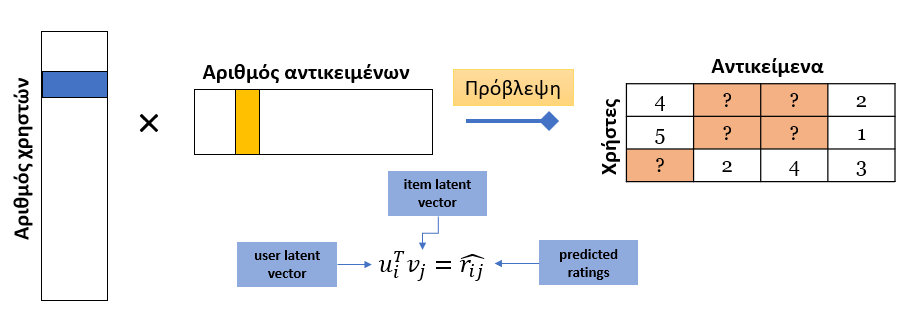
\includegraphics[width=\linewidth]{mf_hand1.png}
\caption{Παραγοντοποίηση μητρώου}
\label{fig:mf}
\end{figure}
Στόχος επομένως, είναι η εύρεση των μητρώων U και V, ώστε να προσεγγίζουν με την καλύτερη δυνατή ακρίβεια το αρχικό μητρώο R. Το κριτήριο για το πόσο καλή είναι μια προσέγγιση δίνεται από μια συνάρτηση κόστους η οποία θα πρέπει να ελαχιστοποιηθεί χρησιμοποιώντας κάποια τεχνική μηχανικής μάθησης. Αυτό είναι ένα κλασικό πρόβλημα ελαχιστοποίησης. Μια επιλογή για τη συνάρτηση κόστους αποτελεί το μέσο τετραγωνικό σφάλμα (Mean Square Error – MSE) λαμβάνοντας υπόψη μόνο τις τιμές που έχουν παρατηρηθεί (observed values):
\\
\qquad\	\qquad\ \qquad\ \qquad\ \[  \min_{\substack{U\in\mathbb{R}^{m\times d},V\in\mathbb{R}^{n\times d}}}{\sum_{i,j\in\mathbb{Z}}\left(R_{ij}-U_iV_j^T\right)^2} 
\]
\\
Αυτό όμως οδηγεί σε συστήματα συστάσεων με αρκετά χαμηλή απόδοση. Μια άλλη σκέψη επομένως είναι να υποθέσουμε ότι οι τιμές που δεν έχουν παρατηρηθεί (unobserved values) είναι ίσες με μηδέν. Σε αυτή την περίπτωση αντί για το μέσο τετραγωνικό σφάλμα στόχος είναι η ελαχιστοποίηση της νόρμας Frobenius ($ ‖·‖^2 $) που είναι ίση με το άθροισμα των τετραγώνων των καταχωρήσεων του μητρώου:\\
\qquad\	\qquad\ \qquad\ \qquad\ \[ \mathop{\min}_{{U \in R^{m \times d}, V \in R^{n \times d}}}||R-UV^\mathsf{T}||^2 \]
\\
Σε ένα πρόβλημα συστάσεων, όπως και σε όλα τα προβλήματα μηχανικής μάθησης, είναι πάντα ορατός ο κίνδυνος της υπερεκπαίδευσης (overfitting) του μοντέλου. Για να το αποφύγουμε αυτό προσθέτουμε στην εξίσωση τον δεύτερο όρο κανονικοποίησης λ που είναι το  L1 regularization και λ είναι η παράμετρος κανονικοποίησης υψωμένης στο τετράγωνο ($ ‖·‖^2 $) \cite{korenMatrixFactorizationTechniques2009}
\begin{align} 
J = \mathop{\min}_{U \in R^{m \times d},V \in R^{n \times d}}{\sum_{i,j\in\mathbb{Z}}\left(R_{ij}-U_iV_j^T\right)^2} + \lambda(||U||_{2} + ||V||_{2}) \label{eq:2}
\end{align} 
Εκτός όμως από την ελαχιστοποίηση της συνάρτησης κόστους, είναι αναγκαίος και ο προσδιορισμός της βέλτιστης τιμής της παραμέτρου κανονικοποίησης λ, καθώς και των βέλτιστων τιμών των i, j. Αυτό μπορεί να γίνει με κάποιον αλγόριθμο βελτιστοποίησης όπως η μέθοδος καθόδου κλίσης (Gradient Descent) η οποία είναι αρκετά δημοφιλής σαν επιλογή, ωστόσο δεν είναι κατάλληλη αν το μητρώο αξιολογήσεων R είναι πολύ μεγάλο, καθώς αυξάνει σημαντικά το υπολογιστικό κόστος. Στη μέθοδο καθόδου κλίσης τα μητρώα U και V  αρχικοποιούνται με τυχαίες τιμές και στη συνέχεια σε κάθε επανάληψη υπολογίζεται το γινόμενο του U με το V και γίνεται η σύγκριση με το αρχικό μητρώο R. Αν το γινόμενο αυτό αποτελεί μια καλή προσέγγιση του R τότε η τρέχουσα επανάληψη τερματίζει, αλλιώς οι τιμές των U και V θα πρέπει να αλλάξουν ώστε να έχουμε μια καλύτερη προσέγγιση του R. Η διαδικασία συνεχίζεται έως ότου φτάσουμε σε κάποιο τοπικό ακρότατο στο εκτιμώμενο σφάλμα ανάμεσα στο μητρώο R και στο εκτιμώμενο μητρώο.\end{itemize}

\noindent \textbf{Μοντέλα βασισμένα στα τεχνητά νευρωνικά δίκτυα}\\
 Τα τελευταία χρόνια ο τεράστιος όγκος των πληροφοριών, σε συνδυασμό με τους περιορισμούς και τα προβλήματα που υπάρχουν στις κλασικές τεχνικές, οδήγησε τους ερευνητές στην υιοθέτηση τεχνικών βαθιάς μάθησης για τη δημιουργία νέων αλγορίθμων συστημάτων συστάσεων. Στο \cite{zhangDeepLearningBased2019} που αποτελεί την πληρέστερη έρευνα που έχει γίνει έως τώρα, συγκεντρώνονται όλες οι τεχνικές βαθιάς μάθησης που χρησιμοποιούνται στα συστήματα συστάσεων. \\\\
\textbf{Μοντέλα βασισμένα στα γραφήματα}\\
Τα τελευταία χρόνια, τα νευρωνικά δίκτυα γράφων (Graph Neural Networks) χρησιμοποιούνται για την επίλυση πολλών προβλημάτων της μηχανικής και της βαθιάς μάθησης. Προτού περιγράψουμε όμως τι είναι ένα Graph Νeural Νetwork και στη συνέχεια εξετάσουμε το πως αυτό χρησιμοποιείται στα συστήματα συστάσεων, χρειάζεται πρώτα να ορίσουμε ορισμένες βασικές έννοιες.
\begin{itemize}
\item \textbf{Γράφημα (graph):} στον χώρο των διακριτών μαθηματικών ένα γράφημα (ή γράφος) G = (V, E) είναι μια δομή η οποία αποτελείται από ένα σύνολο ακμών E και ένα σύνολο κορυφών (ή κόμβων) V \cite{rosenDiscreteMathematicsIts2002}.
\item \textbf{Graph embeddings:} σύμφωνα με τους Goyal και Ferrara \cite{goyalGraphEmbeddingTechniques2018} ένα graph embedding είναι η μετατροπή των στοιχείων των γραφημάτων (ακμές, κορυφές, χαρακτηριστικά) σε διανύσματα, διατηρώντας παράλληλα τις ιδιότητες των γραφημάτων. Κατά αυτόν τον τρόπο μειώνεται η διάσταση κατά 1 και άρα μειώνεται το υπολογιστικό κόστος.
\item\textbf{Αναδρομικά Νευρωνικά Δίκτυα (Recurrent Neural Networks - RNNs):} στα Αναδρομικά  Νευρωνικά Δίκτυα \cite{rumelhartLearningRepresentationsBackpropagating1986} η έξοδος δεν εξαρτάται μόνο από την είσοδο αλλά και από την προηγούμενη έξοδο και εσωτερική κατάσταση του δικτύου. Τα RNNs είναι κατάλληλα για δεδομένα που είναι διατεταγμένα σε μια σειρά, όπως οι χρονοσειρές και όπως είναι δομημένα μπορούν να λειτουργήσουν σε κατευθυνόμενα «γραμμικά» γραφήματα. Κατ' αυτόν τον τρόπο τα RNNs μπορούν να θεωρηθούν ένας ειδικός τύπος GNN, βοηθώντας μας έτσι να τα κατανοήσουμε καλύτερα.
\end{itemize}
Στη βαθιά μάθηση, ένα Graph Neural Network (GNN) \cite{scarselliGraphNeuralNetwork2009} είναι ένας τύπος νευρωνικού δικτύου για την εξαγωγή συμπερασμάτων και γνώσης από δεδομένα που περιγράφονται από γραφήματα. Ένα γράφημα δίνεται ως είσοδος σε ένα GNN αφού πρώτα γίνει η μετατροπή που απαιτείται. Οι κορυφές και οι ακμές των γράφων στα GNNs αναπαριστώνται από διανύσματα και η σύνδεση μεταξύ κορυφών και ακμών από ένα μητρώο γειτνίασης (adjacency matrix). Σε κάθε επανάληψη, κάθε κόμβος C λαμβάνει πληροφορίες (embeddings) από τους γειτονικούς του κόμβους, υπολογίζει το άθροισμά τους και το μεταφέρει στο επόμενο επίπεδο μαζί με το embedding του. Έτσι δημιουργείται ένα νέο embedding, το οποίο περιέχει τις πληροφορίες του κόμβου C μαζί με τις πληροφορίες για τους γειτονικούς του κόμβους. Στην επόμενη επανάληψη ο κόμβοι μαθαίνουν επιπλέον και τις πληροφορίες της γειτονιάς των γειτονικών τους κόμβων (γείτονες 2ης τάξης). Η διαδικασία συνεχίζεται έως ότου οι κόμβοι μάθουν τις πληροφορίες για όλους τους υπόλοιπους κόμβους του γραφήματος. Τέλος, γίνεται η συλλογή όλων των embeddings και η άθροιση τους, δίνοντας μας ένα ενιαίο embedding για όλο το γράφημα. Ο στόχος των GNNs είναι η εκμάθηση αναπαραστάσεων/embeddings των οντοτήτων ή και των κόμβων χρησιμοποιώντας πληροφορίες γειτνίασης. Τα GNNs μπορούν επίσης να χρησιμοποιηθούν για την εκμάθηση αναπαραστάσεων ακμών και γραφημάτων.\\
Στα συστήματα συστάσεων τα Graph Neural Networks οι αλληλεπιδράσεις χρηστών-αντικειμένων (αγορές, κλικς, προσθήκη προϊόντων στο καλάθι, αξιολογήσεις) περιγράφονται από γραφήματα. Αναλυτικότερα, οι χρήστες και τα αντικείμενα αναπαριστώνται από κορυφές και οι αλληλεπιδράσεις από τις ακμές.
\begin{figure}[!htb]
	%\vspace{2px}%
	\centering
	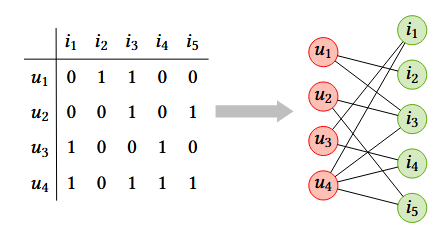
\includegraphics[]{user_item_graph.png}
	\caption[Γράφημα χρηστών-αντικειμένων]{Γράφημα χρηστών-αντικειμένων [Πηγή: \url{https://arxiv.org/pdf/2011.02260.pdf} ]}
	\label{fig:graph}
\end{figure}
\newpage
\subsection{Συστήματα βασισμένα στο περιεχόμενο\\ (Content-based filtering systems)}
\noindent Τα συστήματα βασισμένα στη συνεργατική διήθηση έχουν ως προαπαιτούμενο τη γνώση αλληλεπιδράσεων μεταξύ χρηστών και αντικειμένων. Ένα ερώτημα που γεννάται εδώ, είναι τι συμβαίνει στην περίπτωση που δεν είναι διαθέσιμη αυτή η γνώση. Μια λύση σε αυτό το ζήτημα αποτελούν τα συστήματα βασισμένα στο περιεχόμενο. Τα συστήματα αυτά βασίζονται στα περιγραφικά χαρακτηριστικά των αντικειμένων, όπως το όνομα, η περιγραφή, το είδος κτλ., προκειμένου να δημιουργήσουν νέες συστάσεις. Πιο συγκεκριμένα, σε αυτήν τη μέθοδο οι αλγόριθμοι προτείνουν στον χρήστη παρόμοια αντικείμενα με αυτά που έχει αλληλεπιδράσει στο παρελθόν. Σύμφωνα με τον Falk \cite{falkPracticalRecommenderSystems2019} ένα σύστημα βασισμένο στο περιεχόμενο αποτελείται από τα εξής μέρη:
\begin{enumerate}
	\item Αναλυτής περιεχομένου (Content analyzer) — δημιουργεί ένα μοντέλο βασισμένο στο περιεχόμενο. Κατά μία έννοια, δημιουργεί ένα προφίλ για κάθε αντικείμενο. Σε αυτό το στάδιο γίνεται η προεπεξεργασία των δεδομένων και η μετατροπή τους σε μορφή κατάλληλη για το επόμενο στάδιο και η εκπαίδευση του μοντέλου.
	\item	Δημιουργία προφίλ χρήστη (User profiler) — δημιουργεί το προφίλ ενός χρήστη, με τεχνικές μηχανικής μάθησης. Ορισμένες φορές το προφίλ αυτό αποτελείται από μια απλή λίστα των αντικειμένων που έχει καταναλώσει ο χρήστης.
	\item	Ανάκτηση αντικειμένων (Item retriever) — συγκρίνει τα προφίλ των χρηστών με τα προφίλ των αντικειμένων, με σκοπό την εύρεση και την ανάκτηση σχετικών αντικειμένων για κάθε χρήστη. Εάν το προφίλ του χρήστη είναι μια λίστα αντικειμένων, αυτή η λίστα προσπελαύνεται και βρίσκονται παρόμοια αντικείμενα για κάθε αντικείμενο που υπάρχει στην λίστα του χρήστη. 
\end{enumerate}

\subsection{Υβριδικά συστήματα (Hybrid systems)}
\noindent Τα συστήματα αυτά αποτελούν συνδυασμό των συστημάτων που βασίζονται στο περιεχόμενο και των συστημάτων που βασίζονται στη συνεργατική διήθηση. Το πιο γνωστό παράδειγμα υβριδικού συστήματος είναι το Netflix, το οποίο χρησιμοποιεί μοντέλα συνεργατικής διήθησης για να συγκρίνει τις αναζητήσεις και τις προβολές ταινιών παρόμοιων χρηστών και μοντέλα βασισμένα στο περιεχόμενο για να προτείνει ταινίες που έχουν κοινά χαρακτηριστικά με ταινίες που ο χρήστης έχει δώσει υψηλές αξιολογήσεις.

 \subsection{Προβλήματα στα συστήματα συστάσεων}
 \noindent Σε αυτή την υποενότητα αναφέρονται τα πιο σημαντικά ζητήματα στα συστήματα συστάσεων, τα οποία επηρεάζουν σημαντικά την απόδοση των αλγορίθμων και αποτελούν αιτία εμφάνισης επιπλέον προβλημάτων. Τα ζητήματα αυτά απασχολούν εδώ και πολλά χρόνια την επιστημονική κοινότητα. \\
 
\label{sec:rec_problems}
\noindent \textbf{Χαρακτηριστικά των δεδομένων}\\
Στο \cite{adomaviciusImpactDataCharacteristics2012} και στο \cite{deldjooExplainingRecommenderSystems2021} εξετάζεται το πως τα χαρακτηριστικά των δεδομένων μπορούν να επηρεάσουν την απόδοση των συστημάτων συστάσεων. Ως χαρακτηριστικά των δεδομένων ορίζονται:
\begin{enumerate}
	\item $ \text{\textit{RatingSpace (RS)}} =|U| × |I|  $, το μέγεθος του χώρου των αξιολογήσεων
	\item $ \text{\textit{User Item Ratio (UIR)}} =\frac{|User|}{|Item|} $, ο λόγος χρηστών προς αντικείμενα αποτυπώνει το σχήμα του χώρου αξιολογήσεων.
	\item $  \text{\textit{Rating Per User (RPU)}} = \frac{|Ratings|}{|Users|} $, ο λόγος των αξιολογήσεων προς χρήστες
	\item $ \text{\textit{Rating Per Item (RPI)}} = \frac{|Ratings|}{|Items|} $, ο λόγος των αξιολογήσεων προς αντικείμενα
	\item \textit{Αραιότητα του μητρώου αξιολογήσεων χρηστών-αντικειμένων}, το οποίο αποτελεί ένα πολύ σημαντικό πρόβλημα στα συστήματα συστάσεων και για τον λόγο αυτό αναλύεται περαιτέρω στη συνέχεια
\end{enumerate}
\noindent \textbf{Αραιότητα (Sparsity)}\\
Ένα από τα πιο σημαντικά, αν όχι το πιο σημαντικό, προβλήματα στα συστήματα συστάσεων το οποίο απασχολεί τις τελευταίες δύο δεκαετίες την επιστημονική κοινότητα είναι η αραιότητα των δεδομένων.
Έστω το μητρώο χρηστών-αντικειμένων, το οποίο στις γραμμές περιέχει τους χρήστες και στις στήλες τα αντικείμενα. Κάθε κελί περιέχει την αξιολόγηση ενός χρήστη για ένα αντικείμενο. Για παράδειγμα στην Εικόνα \ref{fig:uimatrix} στο κελί (1,1) βρίσκεται η αξιολόγηση του χρήστη 1 για το αντικείμενο 1 και είναι ίση με 5. 
\begin{figure}[!htb]
	%\vspace{2px}%
	\centering
	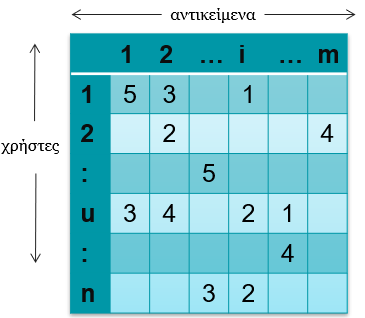
\includegraphics[]{user_item_matrix.png}
	\caption{Παράδειγμα μητρώου χρηστών-αντικειμένων}
	\label{fig:uimatrix}
\end{figure}
Ένα αρκετά σημαντικό ζήτημα που προκύπτει εδώ, είναι πως στις περισσότερες περιπτώσεις το μητρώο αυτό είναι πολύ αραιό, δηλαδή υπάρχουν πολλά κενά κελιά, καθώς καταλαβαίνουμε πως δεν γίνεται όλοι οι χρήστες να έχουν αξιολογήσει όλα τα αντικείμενα σε ένα σύνολο δεδομένων. Η αραιότητα του μητρώου μετριέται σύμφωνα με τον τύπο (με \# συμβολίζεται ο αριθμός):
 \begin{align*}
 	\text{Αραιότητα} = 1 - \frac{\# \text{αξιολογήσεων}}{\# \text{χρηστών} \times \# \text{αντικειμένων}}
 \end{align*}
Συνεπώς, μειώνεται η πιθανότητα να βρεθούν συσχετίσεις ανάμεσα σε χρήστες και αντικείμενα, κάτι που με τη σειρά του οδηγεί σε χαμηλής ποιότητας προβλέψεις. Για τον λόγο αυτό αρκετές είναι οι προσπάθειες τα τελευταία χρόνια να μετριαστεί αυτό το πρόβλημα σε διαφορετικά συστήματα συστάσεων \cite{idrissiSystematicLiteratureReview2020}.
\newpage
 \noindent \textbf{Cold start}\\
 Στα συστήματα συστάσεων απαραίτητη προϋπόθεση είναι η ύπαρξη αρκετών δεδομένων και στοιχείων που να σχετίζονται με τα αντικείμενα και τους χρήστες, προκειμένου να μπορέσουν να βρουν τις απαραίτητες συσχετίσεις ανάμεσα στους χρήστες, στα αντικείμενα και στον συνδυασμό χρηστών και στα αντικειμένων, ώστε να δημιουργήσει συστάσεις προς τους χρήστες με όσο καλύτερη ακρίβεια γίνεται. Ένα ζήτημα που προκύπτει εδώ είναι το λεγόμενο cold start \cite{scheinMethodsMetricsColdstart2002}, το οποίο συμβαίνει κατά κύριο λόγο όταν εισάγεται ένας νέος χρήστης ή ένα νέο αντικείμενο στο σύστημα. Υπάρχουν 3 περιπτώσεις κατά τις οποίες μπορεί να προκύψει αυτό το ζήτημα \cite{brusilovskyAdaptiveWebMethods2007}:
\begin{itemize}
	\item[$\blacksquare$] \textbf{Νέος χρήστης:} όταν ένας χρήστης κάνει εγγραφή στο σύστημα, στην αρχή το σύστημα δεν γνωρίζει τίποτα για εκείνον. Πιο συγκεκριμένα δεν υπάρχει ιστορικό, δηλαδή παλαιότερες αλληλεπιδράσεις όπως αξιολογήσεις που να έχει πραγματοποιήσει σε αντικείμενα, προβολές, κλικ ή αγορές αν πρόκειται για σύστημα ηλεκτρονικού εμπορίου.
	\item[$\blacksquare$] \textbf{Νέο αντικείμενο:} αντίστοιχα όταν ένα νέο αντικείμενο εισάγεται στο σύστημα τότε θα έχει ελάχιστες ή και καθόλου αλληλεπιδράσεις, συνεπώς σύμφωνα με τον τρόπο που λειτουργούν οι αλγόριθμοι συστημάτων συστάσεων, αυτό το αντικείμενο δεν θα προταθεί ποτέ στους χρήστες αν δεν υπάρχουν καθόλου αλληλεπιδράσεις. Εάν υπάρχουν ελάχιστες αλληλεπιδράσεις, τότε η ακρίβεια θα είναι πολύ κακή σε σχέση με τα αντικείμενα με πολλές αλληλεπιδράσεις. Αυτό οδηγεί στο φαινόμενο του popularity bias που περιγράφεται λεπτομερώς σε επόμενα κεφάλαια.
	\item[$\blacksquare$] \textbf{Νέα κοινότητα:} αναφέρεται στην αρχική κατάσταση του συστήματος όπου όλοι οι χρήστες και τα αντικείμενα είναι καινούρια. Στην ουσία είναι ο συνδυασμός των δύο ανωτέρω περιπτώσεων, του νέου χρήστη και του νέου αντικειμένου.
\end{itemize} 
